%%
% 今時jarticleやjbook使ってる人いる?時代はjsarticleかjsbookだよ
% ついでに言うと、uplatexってのはplatexの上位互換、これを使わないなんて旧世代だよね
%
\documentclass[uplatex, report, a4j, 10pt]{jsbook}


%%
% パッケージ群
%
\usepackage{miyazaki-u-paper}   % 宮崎大学工学部の卒論の基本(片山先生作)を、僕がちょっと書き換えちゃった(テヘッ
\usepackage{enumitem}           % enumerate?古い古い
\usepackage[dvipdfmx]{graphicx,hyperref} % 当然dvipdfmなんて使ってないよね
\usepackage{graphicx}
\usepackage[dvipdfmx]{color}    % listingsを使うときにはこれも必須、dvipdfmxを変えちゃうとgraphicxのdvipdfmxも変わるよ
\usepackage{pxjahyper}
\usepackage{listings, jlisting} % コードを埋め込むなら必須
\usepackage{txfonts}            % フォントといえばやっぱりtxfonts、今はnewtxってのもあるらしい
\usepackage{verbatim}           % コメントアウトしてくれる便利なプリアンブルが使える \begin{comment} ... \end{comment}
\usepackage{url}
\usepackage{enumitem}
\usepackage{pdfpages}
% \setlistdepth{6}
% \renewlist{itemize}{itemize}{10}
\hypersetup{
setpagesize=false,
 bookmarksnumbered=true,%
 bookmarksopen=true,%
 colorlinks=true,%
 linkcolor=black,
 citecolor=black,
}
% \usepackage{easy-todo}
\usepackage[hdivide={21mm, , 21mm}, vdivide={30mm, , 25mm}]{geometry} % スタイルを少し変えたくても\hoffset, \voffsetは使わないでね

% todoコマンドを追加
\newcommand\todo[1]{\PackageWarning{Todo}{Detection TODO:#1}\textcolor{red}{(TODO:#1)}}


\renewcommand{\lstlistingname}{コード}
\lstset{
  language={Java},
  frame=tlBR,%フレーム線の指定,上右下左の順,大文字は二重線
%  frameround=tttt,%角の指定,右上|右下|左下|左上の順,tは丸角,fは四角
  framesep=5pt,%本文からframeまでの間隔
  framerule=.2pt,%線の太さ
%  rulecolor={\color[gray]},%線の色
%  backgroundcolor={\color[gray]{.9}},%背景色の指定
  basicstyle={\scriptsize\ttfamily \color[gray]{.15}},%書体の指定,この場合は7ptのタイプライタ体
  identifierstyle={\ttfamily},%識別子の書体
  keywordstyle={\ttfamily \color[cmyk]{0,1,0,0}},%言語ワードの書体
  stringstyle={\scriptsize\ttfamily \color[rgb]{0,0,1}},%文字列リテラルの書体
  commentstyle={\itshape \color[cmyk]{1,0,1,0}},%コメントの書体
  numberstyle={\scriptsize},%行番号の書式
  stepnumber=1,%行番号のステップ間隔
  numbers=left,%行番号の位置
  numbersep=1em,%本文との間隔
  breaklines=true,%改行の設定
  xleftmargin=0zw,
  xrightmargin=0zw,
  columns=[l]{fullflexible},
  lineskip=-0.5zw,
  morecomment={[s][{\color[cmyk]{1,0,0,0}}]{/**}{*/}},
  floatplacement=t,
  classoffset=1,
  showstringspaces=false,%空行の表示
%  breakatwhitespace=true,
%  tabsize=5,
}

\lstdefinestyle{g4}{
  language={C},
  frame=tlBR,%フレーム線の指定,上右下左の順,大文字は二重線
%  frameround=tttt,%角の指定,右上|右下|左下|左上の順,tは丸角,fは四角
  framesep=5pt,%本文からframeまでの間隔
  framerule=.2pt,%線の太さ
%  rulecolor={\color[gray]},%線の色
%  backgroundcolor={\color[gray]{.9}},%背景色の指定
  basicstyle={\scriptsize\ttfamily \color[gray]{.15}},%書体の指定,この場合は7ptのタイプライタ体
  identifierstyle={\ttfamily},%識別子の書体
  keywordstyle={\ttfamily \color[cmyk]{0,1,0,0}},%言語ワードの書体
  stringstyle={\scriptsize\ttfamily \color[rgb]{0,0,1}},%文字列リテラルの書体
  commentstyle={\itshape \color[cmyk]{1,0,1,0}},%コメントの書体
  numberstyle={\scriptsize},%行番号の書式
  stepnumber=1,%行番号のステップ間隔
  numbers=left,%行番号の位置
  numbersep=1em,%本文との間隔
  breaklines=true,%改行の設定
  xleftmargin=0zw,
  xrightmargin=0zw,
  columns=[l]{fullflexible},
  lineskip=-0.5zw,
  morecomment={[s][{\color[cmyk]{1,0,0,0}}]{/**}{*/}},
  floatplacement=t,
  classoffset=1,
  showstringspaces=false,%空行の表示
%  breakatwhitespace=true,
%  tabsize=5,
}


% \lstset{language = modelica,
%         basicstyle=\fontsize{9pt}{10.5pt}\ttfamily,
%         backgroundcolor={\color[gray]{.90}},
%         breakindent = 10pt
%         }
%%
% miyazaki-u-paper.sty用設定値
%
\degree{g} % Graduateのg or Masterのm
\figurenumbering{f} % 図目次を付ける場合はt (真) を持つ真偽値を引数に取る関数
\tablenumbering{f} % 表目次を付ける場合はt (真) を持つ真偽値を引数に取る関数
\title{OpenModelicaのシミュレーション結果を\\用いたモータ特性表自動生成ツールの試作}
\author{原田 海人}
\nendo{元} % 年度
\advisor{片山 徹郎 教授} % 修論では無視する
\major{情報システム工学科}




\begin{document}
\maketitle


%
% 本文
%
\chapter{はじめに}\label{cha:Introduction}
近年、モータは、エアコン・洗濯機・掃除機などの家電製品をはじめ、自動車関係、医療関係など様々な分野に
用いられており\cite{モータ使用製品}、社会に必要不可欠な存在となっている。\\
~はじめに 流れ 案~\\
モータの開発は~で、~の課題がある。それを解決する手段としてシミュレーションがある。
シミュレーションツールの中にOpenModelicaがある。OpenModelicaは~で、~する。
また、結果を画面所にプロットすることで結果を確認できる。
シミュレーションを行った場合、期待通りか結果と比較する。\\
比較する際は、シミュレーション結果から目的のグラフや値を計算等して作成しなければならない。\\
しかし、OpenModelicaではグラフでしか確認できず、具体的な値を取得することが困難である。
そこで、本研究では、モータのシミュレーションをOpenModelicaで行った際のシミュレーション結果の確認にかかる手間を削減することを目的として、
シミュレーション結果のcsvファイルからモータ特性表を自動生成するツールを試作する。\\
% 今回試作したツールで、グラフや値を作成する手間を省くことで、モータ開発の効率化を図る。\\



本論文の構成は、以下の通りである。\\
第2章では、モータ特性表自動生成ツールを試作するために必要となる前提知識について説明する。\\
第3章では、試作したモータ特性表自動生成ツールの構成及び手順について説明する。\\
第4章では、試作したモータ特性表自動生成ツールが正しく動作することを検証する。\\
第5章では、試作したモータ特性表自動生成ツールについて考察する。\\
第6章では、、本論文のまとめとの課題を述べる。\\
\chapter{研究の準備}\label{cha:Preparation}
本章では、本研究で必要となる前提知識を説明する。
% \section{モータ作成}\label{motor}
% \subsection{仕様書}\label{siyo}
% \subsection{シミュレータの役割}\label{simu}
\section{Modelica言語}\label{modelica}
Modelica言語とは、微分代数方程式を用いた、複合領域のマルチドメインモデリングのために開発されたオブジェクト指向言語である\cite{modelicaモデルベース本}。
その言語仕様は、非営利団体のModelica Associationが策定している。
Modelica Associationでは、Modelica言語による様々な物理領域のモデルライブラリを開発しており、
数学、機械、電気、熱、流体、制御系、状態遷移機械などを含んだフリーのModelica標準ライブラリ(Modelica Standard Library : MSL)をリリースしている
\cite{modelicaモデルベース本}。
\section{OpenModelica}\label{OM}
OpenModelicaとは、Open Source Modelica Consortium (OSMC)が開発しているModelicaコードのモデリング、シミュレーション、デバッグのための機能などを
持つオープンソースプラットフォームである\cite{fritzson2006openmodelica}。
OpenModelicaでは、シミュレーション結果をグラフとして画面上に描画できる。また、シミュレーション結果は、以下の3つのファイル形式から保存することができる。
\begin{itemize}
    \item matファイル
    \item pltファイル
    \item csvファイル
\end{itemize}

今回試作するモータ特性表自動生成ツールでは、csvファイルにのみ対応する。

OpenModelicaから出力されるcsvファイルの一部を、図\ref{fig:simyu_csv}に示す。

図\ref{fig:simyu_csv}に示すcsvファイルの1列目には、時間を表すデータが必ず入る。
そして1列目の「time」を除いて1行目には、オブジェクト名を含んだ変数名が必ず入る。

OpenModelicaから出力されるcsvファイルのファイル名は、「(シミュレーションしたモデルの名前)\_res.csv」で生成される。
もし、シミュレーションしたモデルの名前が、「hoge」だった場合、csvファイルのファイル名は「hoge\_res.csv」となる。\\
\begin{figure}[t]
	\centering
	\includegraphics[width=16.5cm,height=10cm]{./Image/simyu_csv.png}
	\caption{シミュレーション結果のcsvファイルの一部}
	\label{fig:simyu_csv}
\end{figure}
% 試作するモータ特性表自動生成ツールでは、OpenModelica 1.9.1 Beta1を使用する。
\section{ブラシ付きDCモータ}\label{}
% ブラシ付きDCモータだけかけばいいのか?モータ全体の話も必要か?
ブラシ付きDCモータとは、磁場の中にあるコイルに電流を流す事で発生するローレンツ力を回転方向に利用することで回すモータである\cite{モータ原理}。
シンプルな構造で、制御しやすく、汎用性が高く、模型用モータや自動車補機用モータなど世界で一番多く使われているモータである\cite{モータ使う}。
% 3章へ
%   今回試作するモータ特性表自動生成ツールでは、ブラシ付きモータのシミュレーション結果にのみ対応する。
\section{対応するモデル}\label{taioumodel}
試作するモータ特性表自動生成ツールでは、以下2つのModelicaモデルのシミュレーション結果に対応する。
% \begin{itemize}
% 	\item ブラシ付きDCモータのModelicaモデル
% 	\item ブラシ付きDCモータのModelicaモデルをサブシステムとするモデル
% \end{itemize}
% 以降、上記のモデルについて具体的に説明する。
\subsection{ブラシ付きDCモータのModelicaモデル}\label{sub:tanntai}
ブラシ付きDCモータのModelicaモデルとは、ブラシ付きDCモータの等価回路\cite{等価回路}をModelica言語で表したモデルのことである。

ブラシ付きDCモータの等価回路をModelica言語で表すためには、電源部品、抵抗部品、インダクタ部品、起電力部品、慣性部品、接地部品が必要である。
% 上記6つの部品が必要な理由は、ブラシ付きDCモータの等価回路\cite{等価回路}をModelica言語で表す際に、使用する部品\cite{modelicaシステム本}だからである。\\

また、電源部品、抵抗部品、インダクタ部品、起電力部品、慣性部品には、それぞれ以下のパラメータを設定しなければならない。
\begin{itemize}
	\item 電源部品 ・・・ 電圧値 V
	\item 抵抗部品 ・・・ 抵抗値 $\Omega$
	\item インダクタ部品 ・・・ インダクタンス値 H
	\item 起電力部品 ・・・ トルク定数 $\mathrm{N\cdot m/A}$
	\item 慣性部品 ・・・ 慣性モーメント $\mathrm{kg\cdot m^2}$
\end{itemize}

各部品で使用するMSLを表\ref{tab:MSL}に、ブラシ付きDCモータの等価回路を図\ref{fig:touka}に、ブラシ付きDCモータのModelicaモデルの例を図\ref{fig:tantai_model}に、
図\ref{fig:tantai_model}のModelicaコードを図\ref{fig:tantai_modelica}に、それぞれ示す。

\begin{table}[t]
	\centering
	\caption{MSL対応表}
	\begin{tabular}{|c|c|} \hline
	  部品名 & 使用するMSL \\ \hline \hline
	  電源部品 & Modelica.Electrical.Analog.Sources \\ \hline
	  抵抗部品 & Modelica.Electrical.Analog.Basic \\ \hline
	  インダクタ部品 & Modelica.Electrical.Analog.Basic \\ \hline
	  起電力部品 & Modelica.Electrical.Analog.Basic \\ \hline
	  慣性部品 & Modelica.Mechanics.Rotational.Components \\ \hline
	  接地部品 & Modelica.Electrical.Analog.Basic \\ \hline
	\end{tabular}
	\label{tab:MSL}
  \end{table}
 
\begin{figure}[t]
	\centering
	\includegraphics[width=7cm]{./Image/touka.png}
	\caption{ブラシ付きDCモータの等価回路}
	\label{fig:touka}
  \end{figure}

\begin{figure}[t]
  \centering
  \includegraphics[width=10cm]{./Image/tantai_model.png}
  \caption{ブラシ付きDCモータのModelicaモデルの例}
  \label{fig:tantai_model}
\end{figure}


% \begin{figure*}[t]
% 	\lstinputlisting[label={code:motor}, caption={図\ref{fig:tantai_model}のModelicaコード}]{./chapters/motor.mo}
% \end{figure*}

\begin{figure}[t]
	\centering
	\includegraphics[width=16.5cm,height=8cm]{./Image/tantai_modelica.png}
	\caption{図\ref{fig:tantai_model}のModelicaコード}
	\label{fig:tantai_modelica}
  \end{figure}

%   \vspace{-1zh}

\subsection{ブラシ付きDCモータのModelicaモデルをサブシステムとするモデル} \label{sub:submodel}
ブラシ付きDCモータのModelicaモデルをサブシステムとするモデルとは、
\ref{sub:tanntai}節で説明したブラシ付きDCモータのModelicaモデルを1つのサブシステムとして扱い、他の部品と合わせたモデルのことである。

例として、ブラシ付きDCモータのサブシステムを用いたDCモータサーボのモデルを図\ref{fig:submodel}に、図\ref{fig:submodel}のModelicaコードを図\ref{fig:sub_modelica}に、それぞれ示す。

\begin{figure}[t]
	\centering
	\includegraphics[width=16.5cm,height=10cm]{./Image/submodel_pack.png}
	\caption{DCモータサーボのモデル}
	\label{fig:submodel}
  \end{figure}

  \begin{figure}[t]
	\centering
	\includegraphics[width=16.5cm,height=10cm]{./Image/sub_modelica.png}
	\caption{図\ref{fig:submodel}のModelicaコード}
	\label{fig:sub_modelica}
  \end{figure}
% 3章へ
%   \subsection{モデル作成時の制約}\label{sub:seiyaku}
%   \ref{sub:tanntai}章、\ref{sub:submodel}章で説明したモデルを作成する際は、以下の制約を満たしていなければならない。
% \subsubsection{電圧値は一定}
% 今回試作するモータ特性表自動生成ツールでは、電圧値が一定の場合に得られる特性\cite{電圧一定}も示すため、入力である電圧値は一定でなければならない。
% \subsubsection{0秒からモータを動かす}
% 今回試作するモータ特性表自動生成ツールの仕様上、モータに対して0秒から入力を与え、モータを動かすようにしなければならない。
\section{モータ特性表}\label{mortoku}
モータ特性表とは、モータを選定する際に、参考にする資料である\cite{仕様の見方}。一般的に決まった形式はなく、企業によって書いている要素は異なるため、
10社のモータ特性表\cite{特性表1,特性表2,特性表3,特性表4,特性表5,特性表6,特性表7,特性表8,特性表9,特性表10}に書かれている要素を集計した。その中でも出現回数が多く、
ブラシ付きDCモータのシミュレーション結果から作成できる要素を、今回自動生成するモータ特性表の要素とした。

以下にモータ特性表の構成と要素を示す。
% \begin{itemize}
% 	\item モータ特性表
% 	\begin{itemize}
% 		\item 特性表
% 		\begin{itemize}
% 			\item 電圧 V
% 			\item 始動電流 mA
% 			\item 停動トルク $mN \cdot m$
% 			\item 最大効率 \%
% 			\item 定格トルク $mN \cdot m$
% 			\item 定格回転数 rpm
% 			\item 定格電流 mA
% 			\item 定格出力 W
% 			\item 最大回転数 rpm 
% 		\end{itemize}
% 		\item 特性グラフ
% 		\begin{itemize}
% 			\item トルク $mN \cdot m$ * 電流 mA
% 			\item トルク $mN \cdot m$ * 回転数 rpm
% 			\item トルク $mN \cdot m$ * 効率 \%
% 			\item トルク $mN \cdot m$ * 出力 W
% 		\end{itemize}
% 	\end{itemize}
% \end{itemize}
\subsection{特性表}\label{sub:tokuseihyou}
特性表を構成する9個の要素が表す内容について述べる。
% \begin{itemize}
% 	\item 電圧 V
% 	\item 始動電流 mA
% 	\item 停動トルク mNm
% 	\item 最大効率 \%
% 	\item 定格トルク mNm 
% 	\item 定格回転数 rpm
% 	\item 定格電流 mA
% 	\item 定格出力 W
% 	\item 最大回転数 rpm 
% \end{itemize}
% 以降、各要素が表す内容について述べる。
\subsubsection{電圧}\label{sub:sub:dennatu}
% \subsection{電圧}\label{sub:dennatu}
電圧とは、シミュレーション時に、回路に印加された電圧値を表す。

単位は、V(ボルト)である。
\subsubsection{始動電流}\label{sub:sub:sidouden}
% \subsection{始動電流}\label{sub:sidouden}
始動電流とは、モータの起動時に流れる電流値を表す。

単位は、mA(ミリアンペア)である。
% https://www.tsugawa.co.jp/glossary/ 
\subsubsection{停動トルク}\label{sub:sub:teidoutoruku}
% \subsection{停動トルク}\label{sub:teidoutoruku}
停動トルクとは、モータが出しうる最大トルクで、このトルク以上の負荷がかかれば、モータが停止する値を表す。

単位は、mNm(ミリニュートンメートル)である。
% https://www.orientalmotor.co.jp/tech/glossary/ta11/
\subsubsection{最大効率}\label{sub:sub:saidaikouritu}
% \subsection{最大効率}\label{sub:saidaikouritu}
効率とは、入力電力に対する機械出力の比を百分率[\%]で表したものであり、最大効率は、その中で最大値を表す。

単位は、\%(パーセント)である。
% https://www.jp-igarashi.com/product/product_motors/curve.html
\subsubsection{定格トルク}\label{sub:sub:teikakutoruku}
% \subsection{定格トルク}\label{sub:teikakutoruku}
定格トルクとは、最大効率時のトルク値を表す。

単位は、mNM(ミリニュートンメートル)である。
% http://www.sagamimicro.co.jp/product/aboutusage.html
\subsubsection{定格回転数}\label{sub:sub:teikakukaiten}
% \subsection{定格回転数}\label{sub:teikakukaiten}
定格回転数とは、最大効率時の回転数値を表す。

単位は、rpm(アールピーエム)である。

% https://mathwords.net/kaitensu
\subsubsection{定格電流}\label{sub:sub:teikakuden}
% \subsection{定格電流}\label{sub:teikakuden}
定格電流とは、最大効率時の電流値を表す。

単位は、mA(ミリアンペア)である。
% http://fa-faq.mitsubishielectric.co.jp/faq/show/18504?category_id=1937&site_domain=default
\subsubsection{定格出力}\label{sub:sub:teikakusyutu}
% \subsection{定格出力}\label{sub:teikakusyutu}
定格出力とは、最大効率時の出力値を表す。

単位は、W(ワット)である。
% \ref{sub:sub:teikakukaiten}章で求めた定格回転数と\ref{sub:sub:teidoutoruku}章で求めた定格トルクを
% http://www.nidec-servo.com/jp/digital/pdf/A_technique.pdf
\subsubsection{最大回転数}\label{sub:sub:saidaikai}
% \subsection{最大回転数}\label{sub:saidaikai}
最大回転数とは、回転数値の中で最大値を表す。

単位は、rpm(アールピーエム)である。
\subsection{特性グラフ}\label{sub:tokuseigurahu}
今回試作したツールでは、以下の4つの特性グラフを作成する。
% \begin{itemize}
% 	\item トルク mNM * 電流 mA
% 	\item トルク mNm * 回転数 rpm
% 	\item トルク mNm * 効率 \%
% 	\item トルク mNm * 出力 W
% \end{itemize}
% 以降、各グラフについて述べる。
\subsubsection{「トルク * 電流」グラフ}\label{sub:sub:torden}
「トルク * 電流」グラフとは、横軸が「トルク mNm」、縦軸が「電流 mA」のグラフである。\\
このグラフでは、トルクに対する電流の変化量を表している。
\subsubsection{「トルク * 回転数」グラフ}\label{sub:sub:torkaiten}
「トルク * 電流」グラフとは、横軸が「トルク mNm」、縦軸が「回転数 rpm」のグラフである。\\
このグラフでは、トルクに対する回転数の変化量を表している。
\subsubsection{「トルク * 効率」グラフ}\label{sub:sub:torkouritu}
「トルク * 電流」グラフとは、横軸が「トルク mNm」、縦軸が「効率 \%」のグラフである。\\
このグラフでは、トルクに対する効率の変化量を表している。
\subsubsection{「トルク * 出力」グラフ}\label{sub:sub:torsyutu}
「トルク * 電流」グラフとは、横軸が「トルク mNm」、縦軸が「出力 W」のグラフである。\\
このグラフでは、トルクに対する出力の変化量を表している。
  \section{Python}\label{python}
Pythonは、1991年にオランダ人のグイド・ヴァンロッサムというプログラマによって開発され、オープンソースで運営されている動的プログラミング言語である\cite{pythonoya}。
一括りにPythonといってもその用途は様々で、組み込み開発や、Webアプリケーション、デスクトップアプリケーション、さらには人工知能開発、ビッグデータ解析などと多岐に渡る\cite{pythonsamu}。
Pythonのプログラミング言語としての主な特徴は、少ないコードで簡潔にプログラムを書けること、専門的なライブラリが豊富にあることなどが挙げられる。

% pythonのバージョンは3.8.0
今回試作するモータ特性表自動生成ツールの開発言語に、Pythonを用いる。
また、使用するライブラリを以下に示す。
\begin{itemize}
	\item csv
	\item math
	\item matplotlib
	\item numpy
	\item decimal
	\item reportlab
	\item PIL
	\item pdf2image
	\item sys
	\item time
	\item os
\end{itemize}
% avaは、1990年代前半にSun MicrosystemsでJames Arthur Gosling、Wiliam Nelson Joyなどの人々が開発したプログラミング言語およびプラットフォームである。
% Javaはクラスベースのオブジェクト指向プログラミング言語である。
% Javaのプログラムは複数のクラスから構成され、クラス定義からそのクラスのインスタンスであるオブジェクトを何個でも作ることができる%\cite{プログラミング言語Java}。

% 1つのjavaファイルには複数のクラスを記述できる。
% 各クラスにはメンバが存在し、メンバの主な種類はフィールドとメソッドである。
% フィールドは、クラス自身あるいはそのクラスのオブジェクトのどちらかに属しているデータ変数である。
% メソッドは、クラスの状態を操作するためにフィールドに対して実行可能な処理を行う振舞いである。

% 今回実装は、で開発する。
%\chapter{モータ特性表自動生成ツール}\label{cha:Tool}
本章では、 本研究で試作したモータ特性表自動生成ツールについて説明する。
モータ特性表自動生成ツールは、モータのシミュレーション結果から、\ref{mortoku}節で述べたモータ特性表を自動生成する。
モータ特性表自動生成ツールの処理の流れを、図\ref{fig:kouzou}に示す。
\begin{figure}[t]
	\centering
	% \includegraphics[width=16.5cm]{./Image/.png}
	\includegraphics[width=14cm]{./Image/kouzou.png}
    \caption{モータ特性表自動生成ツールの構造}
	\label{fig:kouzou}
  \end{figure}
モータ特性表自動生成ツールの入力は、モータに関してシミュレーションしたOpenModelicaから出力されるcsvファイルである。ここで、現時点のツールは、実装上の都合により、入力となるcsvファイルは
次の3つの制約をすべて満たす必要がある。
\begin{itemize}
    \item モータのモデルがブラシ付きDCモータである
    \item モータの回路に印加する電圧値は一定
    \item 0秒からモータに入力を与える
\end{itemize}
モータ特性表自動生成ツールは、3つの処理部で構成しており、それぞれ以下の処理を行う。
\begin{itemize}
    \item csvファイル解析部
    \begin{itemize}
        \item 実行コマンドの取得
        \item csvファイルの読み込み
    \end{itemize}
    \item 特性表の要素算出部
    \begin{itemize}
        \item 基礎データの算出
        \item 特性表の構成要素の算出
    \end{itemize}
    \item モータ特性表生成部
    \begin{itemize}
        \item 特性表の生成
        \item 特性グラフの生成
        \item モータ特性表の生成
    \end{itemize}
\end{itemize}
以降、それぞれの処理部について説明する。
\section{csvファイル解析部}\label{csv_sec}
csvファイル解析部では、モータ特性表自動生成ツールを実行する際のコマンドから、読み込むcsvファイルを決定する。
そして、指定したcsvファイルを読み込み、モータ特性表を生成するために必要なデータを取得する。
以降、各処理について説明する。
\subsection{実行コマンドの取得}\label{sub:comand_get}
読み込むcsvファイルを特定するために、ツールを実行するコマンドの引数に、ファイル名を指定する。
モータ特性表自動生成ツールを実行するためのコマンドを、コード\ref{code:zikkou}に示す。
\begin{figure*}[t]
	\lstinputlisting[label={code:zikkou}, caption={実行コマンド}]{Image/comand.txt}
\end{figure*}
なお、このコマンドは、ツールの実行ファイルが存在するディレクトリで実行する必要がある。

第1引数には、入力とするcsvファイルのパスを含めたファイル名を指定する。

第2引数には、第1引数で指定したcsvファイルの中の、モータ特性表を自動生成したいモータのモデルに含まれる、慣性部品のオブジェクト名を指定する。

第3引数には、第1引数で指定したcsvファイルの中の、モータ特性表を自動生成したいモータのモデルに含まれる、電源部品のオブジェクト名を指定する。

第2引数と、第3引数に慣性部品と電源部品のオブジェクト名を指定する理由については、\ref{sub:csv_scan}節で述べる。

引数を取得するために、コマンドの引数を、1次元の配列で保持するsysライブラリのargvを使用する。
以下に、処理の流れを示す。

\begin{enumerate}
    \item argvの要素数を取得する
    \item 要素数が4以外であれば、図\ref{fig:error_hikisuu}のエラーを表示し、全体の処理を終了する
    \item argvの1番目の要素からファイル名を取得する
    \item 取得したファイル名の拡張子がcsvでない場合、図\ref{fig:error_file}のエラーを表示し、全体の処理を終了する
    \item argvの2番目の要素から慣性部品のオブジェクト名を取得する
    \item argvの3番目の要素から電源部品のオブジェクト名を取得する
\end{enumerate}

\begin{figure}[t]
	\centering
	\includegraphics[width=10cm,height=1.5cm]{./Image/error_tarinai.png}
	\caption{引数の数に誤りがあった場合のエラー文の例}
	\label{fig:error_hikisuu}
\end{figure}
\begin{figure}[t]
	\centering
	\includegraphics[width=12cm,height=1.5cm]{./Image/error_file.png}
	\caption{第1引数に誤りがあった場合のエラー文の例}
	\label{fig:error_file}
\end{figure}
\subsection{csvファイルの読み込み}\label{sub:csv_scan}
モータ特性表の要素を算出するために必要なデータを、csvファイルから取得する。
今回、モータ特性表の自動生成に必要となるデータの導出計算式は、以下の通りである。
% \vspace{3zh}
\begin{itemize}
    \item 効率
    \begin{eqnarray}
         \mbox{効率} = \frac{\mbox{出力}}{\mbox{入力}}  * 100 
        \end{eqnarray}

        \item 出力 
        \begin{eqnarray}
        \mbox{出力} = \mbox{トルク} * \mbox{角速度} 
         \end{eqnarray}
         
        \item 入力  \begin{eqnarray} \mbox{入力} = \mbox{電圧値} * \mbox{電流値} 
    \end{eqnarray}
        \item 回転数  \begin{eqnarray} \mbox{回転数} = \frac{30 * \mbox{角速度}}{\pi}   
    \end{eqnarray}
        \item 定格出力  \begin{eqnarray} \mbox{定格出力} = \mbox{定格トルク} * \mbox{定格回転数} * \frac{2\pi}{60} 
     \end{eqnarray}
     
\end{itemize}


上記の式より、モータ特性表の要素を算出するために必要なデータは、トルク、角速度、電圧、電流であると言える。
また、トルク、角速度、電圧、電流の値を持つcsvファイル内の変数を、表\ref{tab:hensuu}に示す。 
\begin{table}[t]
	\centering
	\caption{各値を持つ変数}
	\begin{tabular}{|c|c|} \hline
	  必要なデータ & 変数 \\ \hline \hline
	  トルク値 & (慣性部品のモジュール名).flange\_a.tau \\ \hline
	  角速度値 &  (慣性部品のモジュール名).w \\ \hline
	  電圧値 &  (電源部品のモジュール名).p.v \\ \hline
	  電流値 &  (電源部品のモジュール名).n.i \\ \hline
	\end{tabular}
	\label{tab:hensuu}
  \end{table}

モータ特性表自動生成ツールで、csvファイルを読み込むために、表\ref{tab:libr}で挙げたcsvライブラリを使用する。csvライブラリを用いた場合、csvファイルを1行ごとに分けて読み込む。
以下に、処理の流れを示す。
\begin{enumerate}
    \item csvファイルを読み込み専用で開く
    \item ファイルが開けなかった場合、図\ref{fig:error_file}のエラーを表示し、全体の処理を終了する
    \item csvファイルの行数分、以下の処理を繰り返す
    \begin{enumerate}
        \item csvファイルから取り出した行を、csvファイルの行の値を保持する配列rowに格納する。
        \item csvファイルの1行目を読み込んでいる場合、配列rowの要素数分、以下の処理を繰り返す
            \begin{enumerate}
                \item 変数名に、慣性部品のオブジェクト名が含まれている場合、以下の処理を行う
                \begin{enumerate}
                    \item 変数名の末尾に、「.flange\_a.tau」が含まれている場合、その変数名を格納している配列rowのインデックスを取得する
                    \item 変数名の末尾に、「.w」が含まれている場合、その変数名を格納している配列rowのインデックスを取得する
                \end{enumerate}
                \item 変数名に、電源部品のオブジェクト名が含まれている場合、以下の処理を行う
                \begin{enumerate}
                    \item 変数名の末尾に、「.p.v」が含まれている場合、その変数名を格納している配列rowのインデックスを取得する
                    \item 変数名の末尾に、「.n.i」が含まれている場合、その変数名を格納している配列rowのインデックスを取得する
                \end{enumerate}
            \end{enumerate}
            \item (a)で配列rowのインデックスを4つ取得するが、いずれか1つでも取得できない場合、図\ref{fig:error_comand}のエラーを表示し、全体の処理を終了する
    \end{enumerate}
        \item csvファイルの2行目を読み込んでいる場合、以下の処理を行う
        \begin{enumerate}
            \item 
        \end{enumerate}
        \item csvファイルの3行目以下を読み込んでいる場合、以下の処理を行う
        \begin{enumerate}
            \item トルク値を格納する配列である配列torqueに、3.(a).i.A.で取得した配列rowのインデックスにある値を格納する
            \item 角速度値を格納する配列である配列angularvelocityに、3.(a).i.B.で取得した配列rorwのインデックスにある値を格納する
            \item 電圧値を格納する配列である配列voltageに、3.(a).ii.A.で取得した配列rowのインデックスにある値を格納する
            \item 電流値を格納する配列である配列currentに、3.(a).ii.B.で取得した配列rowのインデックスにある値を格納する
        \end{enumerate}
\end{enumerate}
% なお、上記の処理の流れにおいて、
% csvファイルの2行目を読み込まない理由は、\ref{OM}節で述べたように、2行目にはモデルを作成した際の初期値が格納されており、初期値はモータ特性表の要素を算出することに使用しないからである。
\begin{figure}[t]
	\centering
	\includegraphics[width=12cm,height=1.5cm]{./Image/error_comand.png}
	\caption{第2引数、第3引数に誤りがあった場合のエラー文の例}
	\label{fig:error_comand}
\end{figure}
\section{特性表の要素算出部}\label{youso_sec}
特性表の要素算出部では、\ref{csv_sec}節で取得したデータをもとに、特性表の各要素を算出する。
まず、特性表の各要素を算出するために必要となる基礎データを算出する。基礎データとは、回転数、出力、効率の値のことを指す。
そして、\ref{csv_sec}節で取得したデータと基礎データから特性表の各要素を算出する。
以降、各処理について説明する。
\subsection{基礎データの算出}\label{sub:youso_kiso}
基礎データの算出処理では、回転数、出力、効率の値を持つ配列を、それぞれの値に対して生成する。
生成方法を以下に示す。
\subsubsection{回転数}\label{sub:sub:kaiten}
% 回転数を算出する式は、\ref{sub:csv_scan}節の箇条書き中にある、回転数にて示した式を用いる。
回転数を算出する式は、\ref{sub:csv_scan}節の(3.4)式を用いる。
配列angularvelocityから、配列の要素数分、繰り返し処理で、回転数の値を持つ配列speedを生成する。
\subsubsection{出力}\label{sub:sub:syutu}
% 出力を算出する式は、\ref{sub:csv_scan}節の箇条書き中にある、出力にて示した式を用いる。
出力を算出する式は、\ref{sub:csv_scan}節の(3.2)式を用いる。
配列torqueと、配列angularvelocityから、配列の要素数分、繰り返し処理で、出力の値を持つ配列outputを生成する。
\subsubsection{効率}\label{sub:sub:kouritu}
% 効率を算出する式は、\ref{sub:csv_scan}節の箇条書き中にある、効率にて示した式と入力にて示した式を用いる。
効率を算出する式は、\ref{sub:csv_scan}節の(3.1)式と、(3.3)式を用いる。
まず、配列voltageと、配列currentから、(3.3)式を用いて入力値を求める。
そして、配列outputと、求めた入力値から、配列の要素数分、繰り返し処理で、効率の値を持つ配列efficiencyを生成する。
\subsection{特性表の各要素の算出}\label{sub:youso_mortoku}
特性表の各要素の算出処理では、\ref{sub:tokuseihyou}節で述べた9つの要素を算出する。
それぞれの算出方法を以下に示す。
\subsubsection{電圧}\label{sub:sub:dennatu}
モータ特性表自動生成ツールが対応するモデルでは、電圧値が一定のため、配列voltageの要素はすべて同じ値になる。今回は、0番目の値を電圧とする。
\subsubsection{始動電流}\label{sub:sub:sidouden}
始動電流とは、モータの起動時に流れる大きな電流であり、モータが起動した後は逆起電力が発生するため、モータ・コイル部分にかかる電圧が下がり、電流値も下がる。
したがって、配列currentの要素の最大値を始動電流とする。
\subsubsection{停動トルク}\label{sub:sub:teidoutoruku}
停動トルクとは、モータが出しうる最大のトルク値である。したがって、配列torqueの最大値を停動トルクとする。
\subsubsection{最大効率}\label{sub:sub:saidaikouritu}
配列efficiencyの最大値を最大効率とする。
\subsubsection{定格トルク}\label{sub:sub:teikakutoruku}
定格トルクとは、最大効率時のトルク値である。まず、配列efficiencyの中で、最大効率である要素のインデックスを取得する。
そして、配列torqueの中で、取得した最大効率のインデックスと同じ位置にある値を定格トルクとする。
\subsubsection{定格回転数}\label{sub:sub:teikakukaiten}
定格回転数とは、最大効率時の回転数の値である。配列speedの中で、取得した最大効率のインデックスと、同じ位置にある値を定格回転数とする。
\subsubsection{定格電流}\label{sub:sub:teikakuden}
定格電流とは、最大効率時の電流値である。配列currentの中で、取得した最大効率のインデックスと、同じ位置にある値を定格電流とする。
\subsubsection{定格出力}\label{sub:sub:teikakusyutu}
定格出力とは、定格動作点における出力の値である。定格出力を算出する式は、\ref{sub:csv_scan}節の(3.5)式を用いる。
上記の定格トルクと定格回転数で求めた値を、定格出力を算出する式に代入し、得た値が定格出力である。
\subsubsection{最大回転数}\label{sub:sub:saidaikai}
最大回転数とは、配列speedの最大値を最大回転数とする。
\section{モータ特性表生成部}\label{mortoku_sec}
モータ特性表生成部では、\ref{csv_sec}節と\ref{youso_sec}節で算出した要素を用いて、モータ特性表を自動生成する。まず、特性表を生成し、画像として保存する。
次に、\ref{sub:tokuseigurahu}節で挙げた4つの特性グラフを生成し、画像として保存する。最後に、特性表の画像と、特性グラフの画像をPDFファイルに書き込むことで、モータ特性表を自動生成する。
以降、各処理について説明する。
\subsection{特性表生成}\label{sub:mortortoku}
この処理では、\ref{sub:youso_mortoku}節で作成した特性表の要素の配列を用いて、特性表を生成する。処理の流れを以下に示す。
\begin{enumerate}
    \item 特性表の各要素の名前を持つ配列を作成する(コード\ref{code:name}参照)
    \item 特性表の要素の配列と、特性表の各要素の名前を持つ配列から、特性表用の配列を作成する
    \item 特性表用の配列から特性表を生成し、生成した表の上部に「モータ特性表」の文字を追加し、画像として保存する。
\end{enumerate}
上記の処理で生成した特性表の画像を、図\ref{fig:toku_gazou}に示す。
\begin{figure*}[t]
	\lstinputlisting[label={code:name}, caption={特性表を構成する要素名の配列}]{Image/name.txt}
\end{figure*}
\begin{figure}[t]
	\centering
	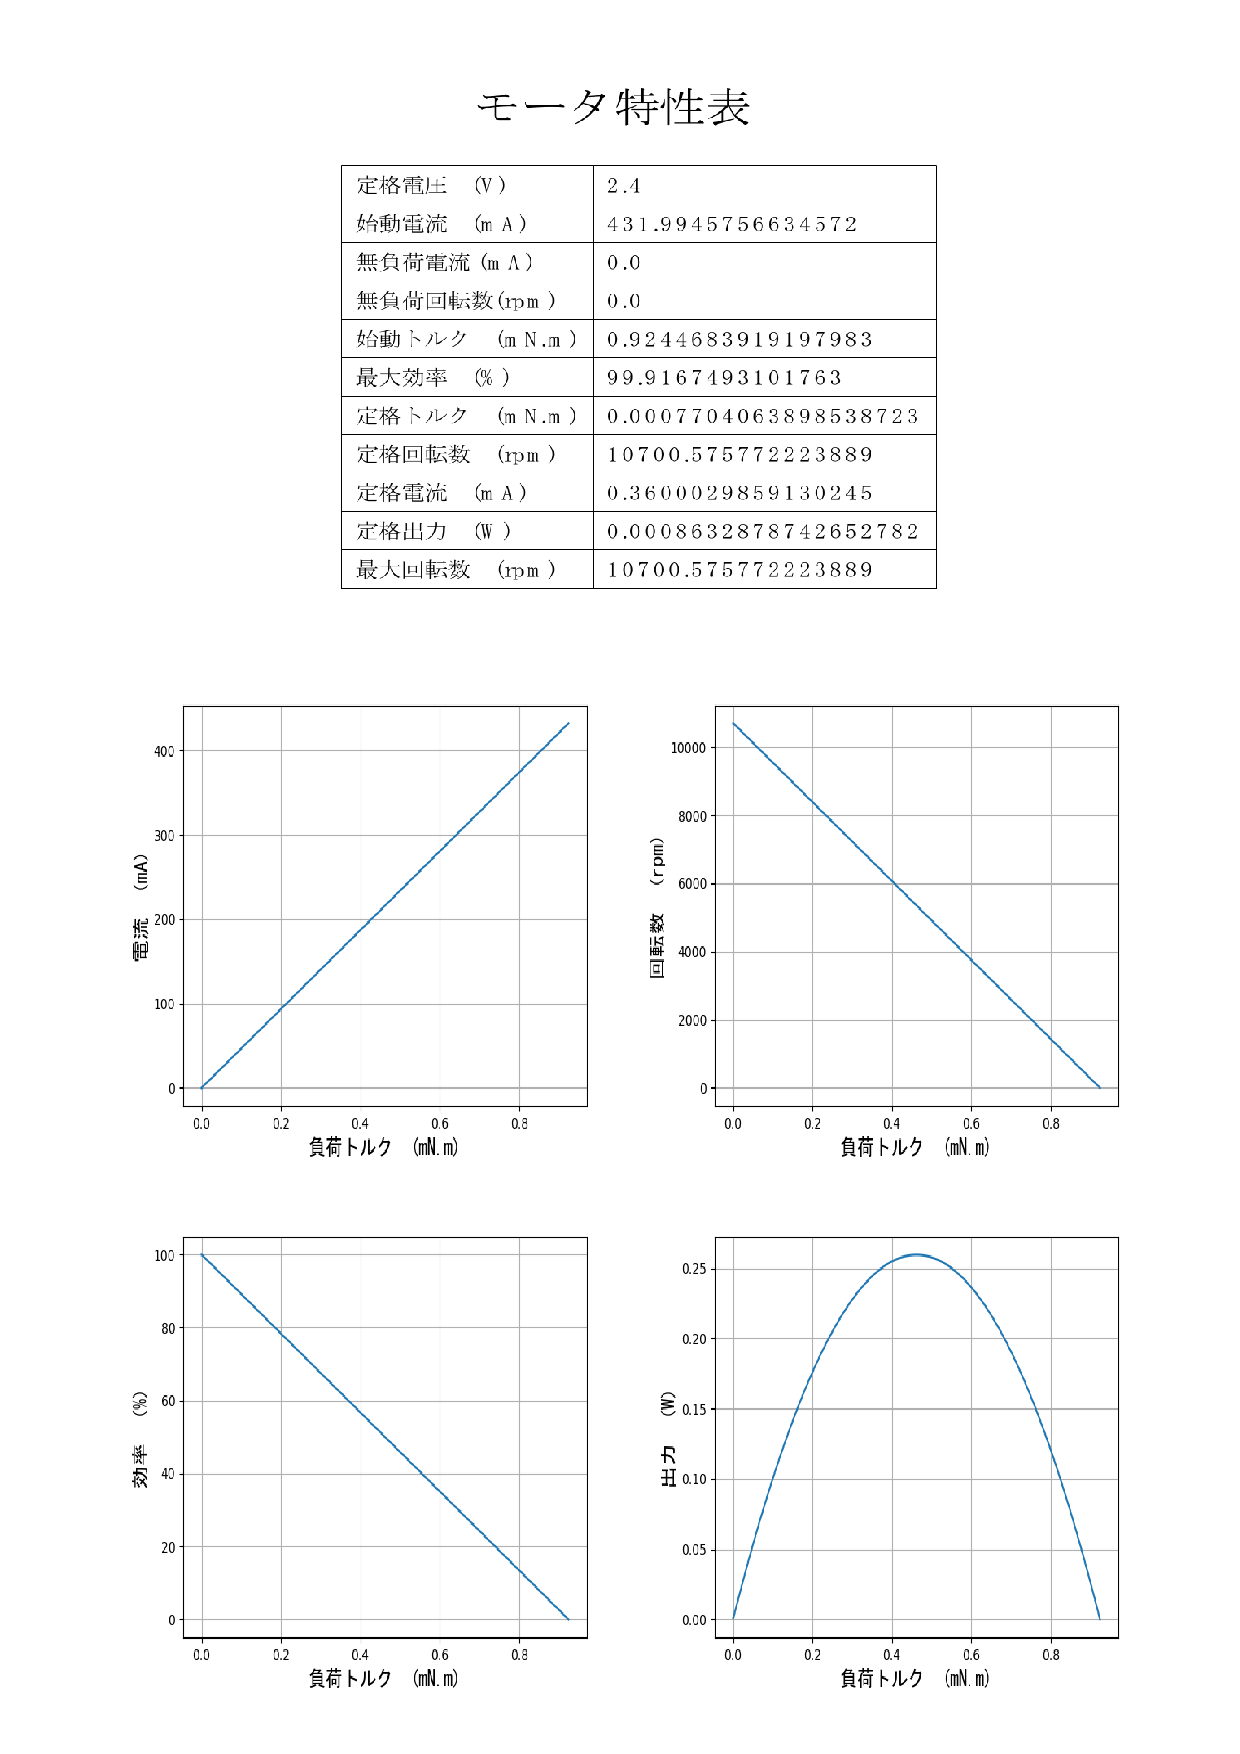
\includegraphics[width=7cm]{./Image/characteristicTable.png}
	\caption{特性表の画像}
	\label{fig:toku_gazou}
\end{figure}
\subsection{特性グラフ生成}\label{sub:toku_gurahu}
\ref{sub:csv_scan}節、\ref{sub:youso_kiso}節で求めた要素の配列を用いて、特性グラフを生成する。
処理の流れを以下に示す。
\begin{enumerate}
    \item x軸にトルク値を持つ配列を、y軸に電流値を持つ配列を指定してグラフを生成し、画像として保存する
    \item x軸にトルク値を持つ配列を、y軸に回転数値を持つ配列を指定してグラフを生成し、画像として保存する
    \item x軸にトルク値を持つ配列を、y軸に効率値を持つ配列を指定してグラフを生成し、画像として保存する
    \item x軸にトルク値を持つ配列を、y軸に出力値を持つ配列を指定してグラフを生成し、画像として保存する
\end{enumerate}
上記の処理で生成した4つのグラフを、それぞれ図\ref{fig:current}、図\ref{fig:speed}、図\ref{fig:effi}、図\ref{fig:output}に示す。
\begin{figure}[t]
	\centering
	\includegraphics[width=7cm]{./Image/current.png}
	\caption{「トルク * 電流」グラフ}
	\label{fig:current}
\end{figure}
\begin{figure}[t]
	\centering
	\includegraphics[width=7cm]{./Image/speed.png}
	\caption{トルク * 回転数」グラフ}
	\label{fig:speed}
\end{figure}
\begin{figure}[t]
	\centering
	\includegraphics[width=7cm]{./Image/efficiency.png}
	\caption{「トルク * 効率」グラフ}
	\label{fig:effi}
\end{figure}
\begin{figure}[t]
	\centering
	\includegraphics[width=7cm]{./Image/output.png}
	\caption{「トルク * 出力」グラフ}
	\label{fig:output}
\end{figure}
\subsection{モータ特性表生成}\label{sub:}
\ref{sub:mortortoku}節と、\ref{sub:toku_gurahu}節で生成した合計5つの画像を、PDFファイルに書き込み、モータ特性表を自動生成する。
モータ特性表のPDFファイルのファイル名は、「characteristicTable.pdf」で生成する。同じファイル名がある場合、上書き保存する。
この処理で自動生成するモータ特性表を、図\ref{fig:tokuseihyou}に示す。
\begin{figure}[t]
	\centering
	\fbox{
	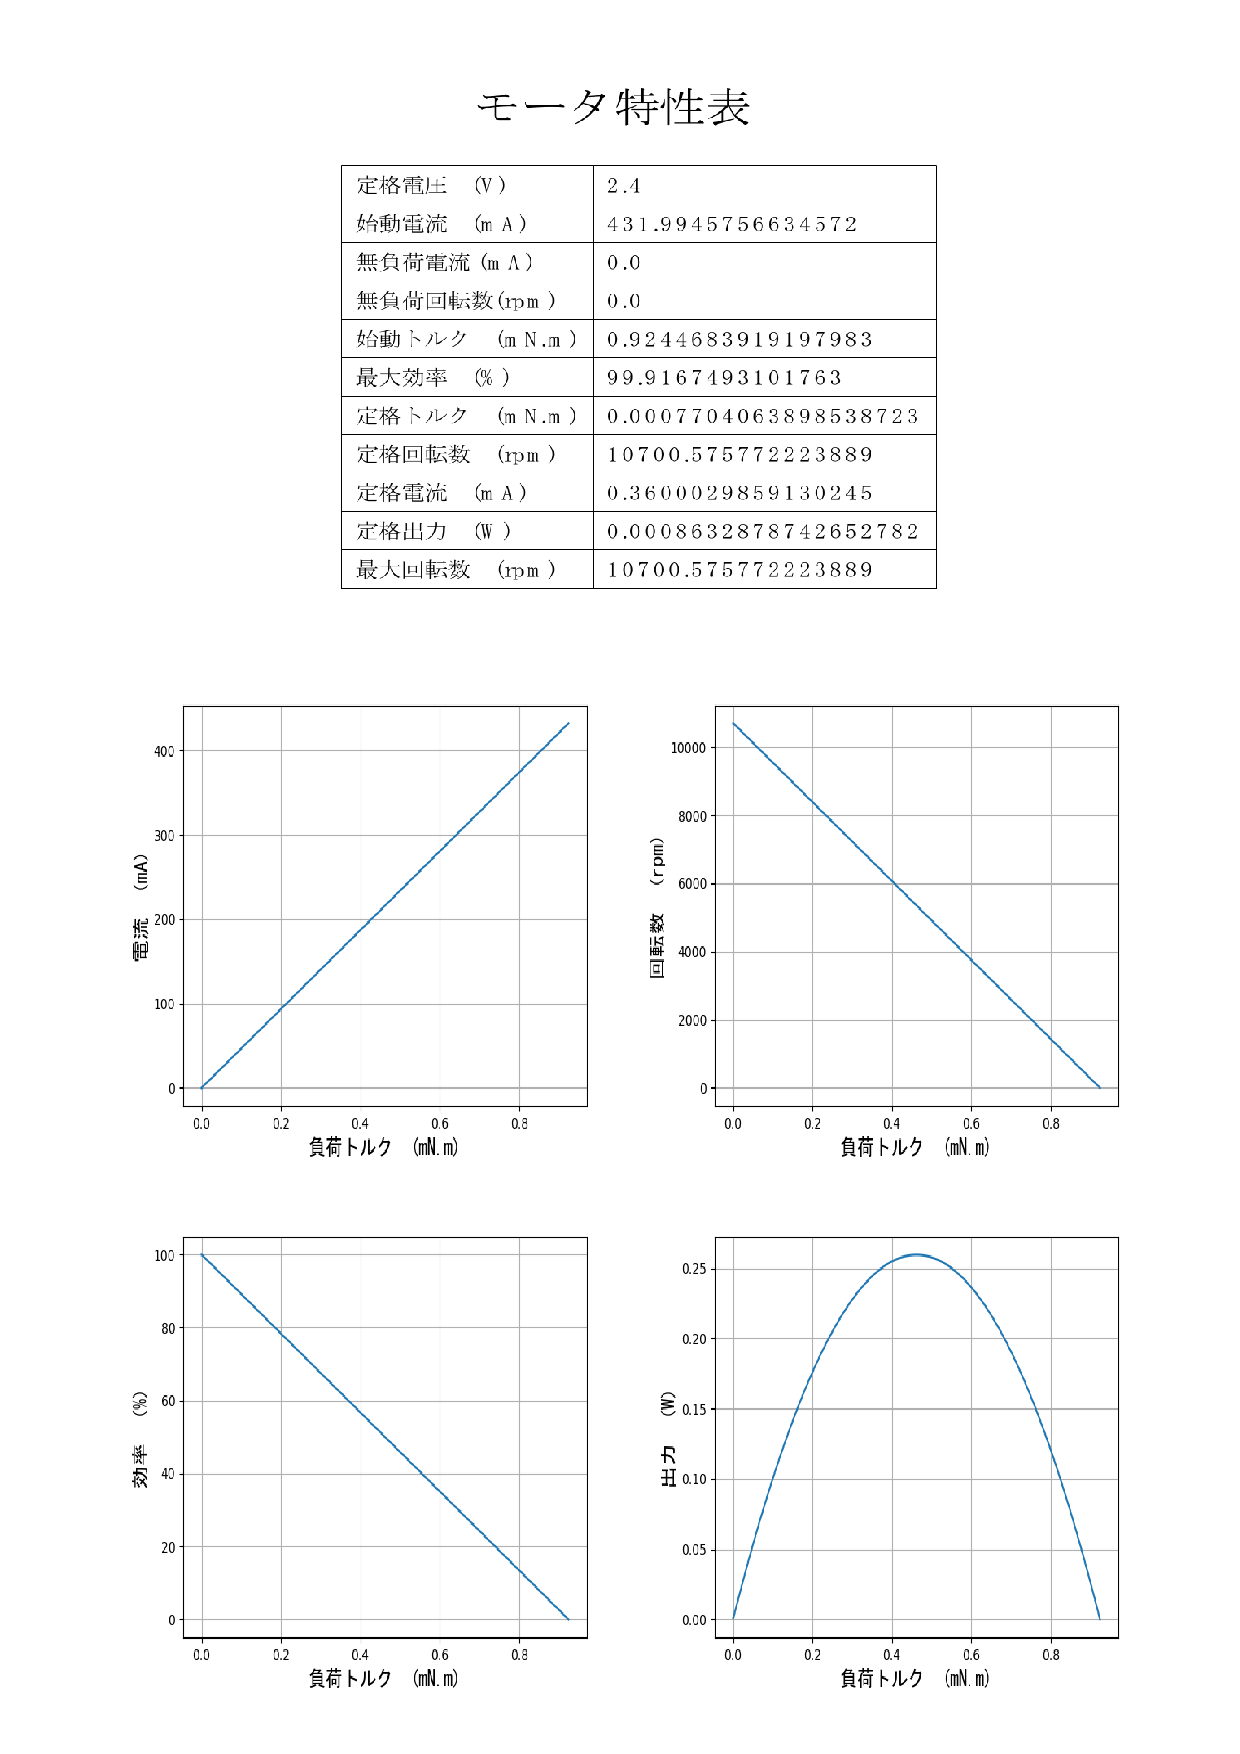
\includegraphics[width=16cm,pagebox=cropbox]{Image/characteristicTable.pdf} 
	}
	\caption{モータ特性表}
	\label{fig:tokuseihyou}
\end{figure}
% \chapter{機能}\label{cha:Function}

本章では、本研究で試作したモータ特性表自動生成ツールの機能について説明する。\\

モータ特性表自動生成ツールは、OpenModelicaで、Modelica言語にて作成したモータの
モデルを、シミュレーションした時に出力されるcsvファイルを読み込み、実行することによって、モータ特性表を生成する。\\

\section{対応するモデル}\label{taioumodel}
試作したモータ特性表自動生成ツールでは、以下のModelicaモデルのシミュレーション結果に対応する。
\begin{itemize}
	\item モータ単体のModelicaモデル
	\item モータ単体のModelicaモデルをサブシステムとするモデル
\end{itemize}
なお、今回はモータの中でもブラシ付きDCモータに対応する。\\
以降、上記のモデルについて具体的に説明する。

\subsection{モータ単体のModelicaモデル}\label{sec:sub1}
モータ単体のModelicaモデルとは、電源部品、抵抗部品、インダクター部品、起電力部品、慣性部品、接地部品を
持つモデルのことである。\\
上記6つの部品が必要な理由は、ブラシ付きDCモータの等価回路\cite{等価回路}をModelica言語で表す際に
使用する部品\cite{modelicaシステム本}だからである。\\
ブラシ付きDCモータの等価回路を図\ref{fig:touka}に、モータ単体のModelicaモデルを図\ref{fig:tantai_model}に、
モータ単体のModelicaモデルをModelicaコードで表したものを図\ref{fig:tantai_modelica}に示す。

\begin{figure}[t]
	\centering
	\includegraphics[width=10cm]{./Image/touka.png}
	\caption{等価回路}
	\label{fig:touka}
  \end{figure}

\begin{figure}[t]
  \centering
  \includegraphics[width=10cm]{./Image/tantai_model.png}
  \caption{モータ単体のModelicaモデル}
  \label{fig:tantai_model}
\end{figure}

\begin{figure}[t]
	\centering
	\includegraphics[width=16.5cm,height=8cm]{./Image/tantai_modelica.png}
	\caption{モータ単体のModelicaモデルのModelicaコード}
	\label{fig:tantai_modelica}
  \end{figure}

\subsection{モータ単体のModelicaモデルをサブシステムとするモデル}\label{sec:sub2}
モータ単体のModelicaモデルをサブシステム\cite{modelicaシステム本}(準備に書く?)とするモデルとは、\ref{sec:sub1}節で説明した
モータ単体のModelicaモデルを一つのモデルにして、サブシステムとして書いたモデルのことである。\\
例を図\ref{fig:subsisu_modelica}に示す。

\begin{figure}[t]
	\centering
	\includegraphics[width=16.5cm,height=8cm]{./Image/tantai_modelica.png}
	\caption{モータ単体のModelicaモデルをサブシステムとするモデル}
	\label{fig:subsisu_modelica}
  \end{figure}


\section{モータ特性表生成}\label{kenkyu_mokuteki}
今回試作したモータ特性表自動生成ツールは次の9個の要素を持つモータ特性表を生成する。

\begin{itemize}
	\item 電圧
	\item 始動電流
	\item 停動トルク
	\item 最大効率
	\item 定格トルク
	\item 定格回転数
	\item 定格電流
	\item 定格出力
	\item 最大回転数 
\end{itemize}


% \chapter{実装}\label{cha:Implementation}
本章では、本研究で試作したモータ特性表自動生成ツールの実装について説明する。\\
% 本章では、本研究で試作したモータ特性表自動生成ツールの機能である、「モータ特性表生成機能」、「ツールの実行機能」、「エラー表示機能」の実装について説明する。\\
% \section{特性表生成機能}\label{tokuseihyou_seisei}
% モータ特性表自動生成ツールの処理の流れを図\ref{fig:syori}に示す。\\
% \begin{figure}[t]
% 	\centering
% 	\includegraphics[width=16.5cm,height=10cm]{./Image/sample.png}
% 	\caption{モータ特性表自動生成ツールの処理の流れ}
% 	\label{fig:syori}
%   \end{figure}
% \section{モータ特性表生成機能}\label{tokuseisei}
モータ特性表自動生成機能の処理の流れを以下に示す。
\begin{enumerate}
    \item 実行コマンドを取得する
    \item 第1引数で指定されたcsvファイルを読み込む
    \item 第2引数、第3引数で指定したモジュール名が持つデータを、csvファイルから取得する
    \item モータ特性表の各要素を算出する
    \item 特性表を作成する
    \item 特性グラフを作成する
    \item モータ特性表を生成する
\end{enumerate}

以下、各処理について具体的に説明する。

\section{実行コマンドの引数の取得}\label{comandget}
この処理では、Pythonスクリプトに渡されたコマンドライン引数のリストであるsys.argvで引数を取得し、エラーの検出を行う。
処理の流れを以下に示す。
\begin{enumerate}
    \item sys.argvの要素数を取得する
    \item 要素数が4以外であれば、図\ref{fig:error_hikisuu}のエラーを表示する
    \item sys.argvの1番目のデータを、ファイル名を保存するために用意した変数に格納する
\end{enumerate}

\section{csvファイルの読み込み}\label{csvfairu}
Pythonで実装するため、Pythonの標準ライブラリのcsvモジュールをインポートし、
csvファイルを読み込む。
以下の条件の時に、オブジェクト名が間違っていると判断する。

エラーは、
以下の条件の1つにでも該当した場合、ファイル名が間違っていると判定し、エラー文を画面上に出力する。
\begin{itemize}
    \item ファイルの拡張子が「.csv」ではない
    \item ファイルを開く際にエラーが出たとき
\end{itemize}

\section{第2引数、第3引数で指定されたモジュールが持つデータを、csvファイルから取得}\label{syutoku_data}
\ref{csvfairu}節で読み込んだcsvファイルから、以下のデータを取得する。

\begin{itemize}
    \item 電流
    \item 電圧
    \item トルク
    \item 角速度
\end{itemize}

\ref{OM}節で述べたように、OpenModelicaから出力されたcsvファイルの1行目には、
各部品のモジュール名を含んだ変数名が記載されている。これを利用して、次の処理で必要なデータを取得する。

\begin{enumerate}
    \item 取得したいデータを持つ変数名を検索する
    \item 変数名のある場所の添字を取得する
    \item 各データごとに用意した配列に、にある値を格納する
    \item 
    \item あ
    \item csvファイルが読み終わるまでーーの処理を繰り返し行う
\end{enumerate}
!!!取得したいデータを持つ変数名を探し、その変数名がある場所の添字を取得する。
各データごとに用意した配列に、同じ添字の位置にある値を繰り返し処理で格納する方法でそれぞれの値を取得する。
アルゴリズムっぽく


以下の条件の1つにでも該当した場合、指定したオブジェクト名が間違っていると判定し、エラー文を画面上に出力する。
\begin{itemize}
    \item 電流値のある添え字を持つ変数が、初期値である「0」であった場合
    \item 電圧のある添え字を持つ変数が、初期値である「0」であった場合
    \item トルクのある添え字を持つ変数が、初期値である「0」であった場合
    \item 角速度のある添え字を持つ変数が、初期値である「0」であった場合
\end{itemize}

\section{モータ特性表の各要素を算出する}\label{keisan}
\ref{syutoku_data}節で取得したデータを用いて、\ref{kenkyu_mokuteki}節で挙げた各要素の値を求める。

\subsection{電圧}\label{sub:keisan_dennatu}
% シミュレーション時に印加した値を取る。
今回試作したツールでは、電源部品の電圧値を電圧とする。

\subsection{始動電流}\label{sub:keisan_sidouden}
% 始動電流とは、モータの起動時に流れる大きな電流のことである。
% モータが起動した後はモータ自体が発電機にもなり、逆起電力を発生するため、モータ・コイル部分にかかる電圧が下がり、電流値も下がる。
% したがって、電流値の配列の中で一番大きい値を始動電流とする。
モータが起動した後は、逆起電力を発生させるため、モータ・コイル部分にかかる電圧が下がり、電流値も下がる。\\
したがって、今回試作したツールでは、電流値の中で一番大きい値を始動電流とする。
% https://www.tsugawa.co.jp/glossary/ 

\subsection{停動トルク}\label{sub:keisan_teidoutoruku}
% 停動トルクとは、モータが出しうる最大トルクで、このトルク以上の負荷がかかれば、モータは停止する値となる。
% したがって、トルク値の配列の中で一番大きい値を停動トルクとする。
したがって、今回試作したツールでは、トルク値の中で一番大きい値を停動トルクとする。

% https://www.orientalmotor.co.jp/tech/glossary/ta11/

\subsection{最大効率}\label{sub:keisan_saidaikouritu}
効率は以下の式で算出する。

\[
    \mbox{効率} = \frac{\mbox{出力}}{\mbox{入力}}  * 100 
\]
\[
    \mbox{出力} = \mbox{角速度} * \mbox{トルク} 
\]
\[  
    \mbox{入力} = \mbox{電圧} * \mbox{電流} 
\]

今回試作したツールでは、効率値の中で一番大きい値を最大効率とする。


% https://www.jp-igarashi.com/product/product_motors/curve.html

\subsection{定格トルク}\label{sub:keisan_teikakutoruku}
% 最大効率時のトルクを定格トルクという。
したがって、トルク値の配列の中で、最大効率のある効率値の配列の添字と同じ位置にある値が定格トルクとなる。


% http://www.sagamimicro.co.jp/product/aboutusage.html

\subsection{定格回転数}\label{sub:keisan_teikakukaiten}
% 最大効率時の回転数を定格回転数という。
回転数は以下の式で算出できる。

\[
    \mbox{回転数} = \frac{30 * \mbox{角速度}}{\pi}   
\]

したがって、一度繰り返し処理で角速度を回転数に変換し、回転数値の配列の中で、最大効率のある効率値の配列の添字と同じ
位置にある値が定格回転数となる。

% https://mathwords.net/kaitensu

\subsection{定格電流}\label{sub:keisan_teikakuden}
% 定格電流とは、モータに定格トルクがかかっているときの電流値である。
したがって、電流値の配列の中で、定格トルクのあるトルク値の配列の添字と同じ位置にある値が定格電流となる。

% http://fa-faq.mitsubishielectric.co.jp/faq/show/18504?category_id=1937&site_domain=default

\subsection{定格出力}\label{sub:keisan_teikakusyutu}
% 定格出力とは、定格動作点における出力の値である。
定格出力は以下の式で算出できる。

\[  \mbox{定格出力} = \mbox{定格トルク} * \mbox{定格回転数} * \frac{2\pi}{60} \]
% \ref{sub:keisan_teikakukaiten}章で求めた定格回転数と\ref{sub:keisan_teidoutoruku}章で求めた定格トルクを
% http://www.nidec-servo.com/jp/digital/pdf/A_technique.pdf

\subsection{最大回転数}\label{sub:keisan_saidaikai}
今回試作したツールでは、回転数地の配列の中から一番大きい値を

\section{特性表を作成}\label{sakusei_hyou}
\ref{keisan}章で求めた各値と、\ref{kenkyu_mokuteki}章で挙げた各要素を、
電圧から順に","で区切りつつ特性表生成配列に格納する。そして特性表生成配列を用いてcsvファイルを作成する。


\section{特性グラフを作成}\label{sakusei_gura}


\section{モータ特性表を生成}\label{seisei_mort}



%\chapter{適用例}\label{cha:Indication}
本章では、本研究で作成したテスト支援ツールが正しく動作することを検証する。テスト支援ツールは次に示す10個の機能を持つ。

\begin{itemize}
	\item キャラクター情報入力機能
	\item オブジェクト増減機能
	\item オブジェクト情報入力機能
	\item オブジェクト位置確認機能
	\item ゲームスタートボタン機能
	\item リプレイボタン機能
	\item Warning判定出力機能
	\item 入力キーとタイミングの記録機能
	\item リプレイ機能
	\item エラーメッセージ出力機能
\end{itemize}

この中の、「キャラクター情報入力機能」、「オブジェクト増減機能」、「オブジェクト情報入力機能」、「オブジェクト位置確認機能」、「Warning判定出力機能」、「入力キーとタイミングの記録機能」、
「リプレイ機能」、「エラーメッセージの出力機能」の8個の機能について検証を行う。

なお、「ゲームスタートボタン機能」については、「Warning判定出力機能」と「入力キーとタイミングの記録機能」を実行する前に押下するボタンの機能のため、これらが機能することで、正しく動作したとする。
また、「リプレイボタン機能」については、「リプレイ機能」を実行する前に押下するボタンの機能のため、「リプレイ機能」が機能することで、正しく動作したとする。

\section{モータ単体のモデル}
テスト支援ツールにおいて「キャラクター情報入力機能」が機能することを検証するために、「キャラクター情報を入力する前のキャラクター情報入力ウィンドウ」と、「キャラクター情報を入力した後のキャラクター情報入力ウィンドウ」のキャラクター情報入力ウィンドウを比較する。
キャラクター情報を入力する前のキャラクター情報入力ウィンドウを図5.1に、キャラクター情報を入力した後のキャラクター情報入力ウィンドウを図5.2に、それぞれ示す。
また、入力したキャラクター名とキャラクターのファイルパスを保存しているcsvファイルを、図5.3に示す。

% % \begin{figure}
% % 	\begin{minipage}[t]{0.5\columnwidth}
% % 		\begin{center}
% % 			\includegraphics[clip, width=0.8\columnwidth]{./Image/5.1.eps}
% % 		\end{center}
% % 		\caption{キャラクター情報を入力する前の \protect\newline キャラクター情報入力ウィンドウ}
% % 		\label{fig:left}
% % 	\end{minipage}%
% % 	\begin{minipage}[t]{0.5\columnwidth}
% % 		\begin{center}
% % 			\includegraphics[clip, width=0.8\columnwidth]{./Image/5.2.eps}
% % 		\end{center}
% % 		\caption{キャラクター情報を入力した後の \protect\newline キャラクター情報入力ウィンドウ}
% % 		\label{fig:right}
% % 	\end{minipage}
% % \end{figure}

% % \begin{figure}
% %   \centering
% %   \includegraphics[width=10cm]{./Image/5.3.eps}
% %   \caption{入力したキャラクター名とキャラクターのファイルパスを保存しているcsvファイル}
% % \end{figure}

% キャラクター情報を入力する前のキャラクター情報入力ウィンドウと、キャラクター情報を入力した後のキャラクター情報入力ウィンドウを比較すると、キャラクター画像(ball.jpg)とキャラクター名(Player)を
% 入力できている。また、csvファイルの1行目に、キャラクター名(Player)とキャラクター画像(ball.jpg)のファイルパスが記述していることが
% わかる。よって、「キャラクター情報入力機能」が正しく動作していることを確認できる。

\section{パッケージ化されたモデル}
% テスト支援ツールにおいて、「オブジェクト増減機能」が機能することを検証するために、「オブジェクトを追加する前」と、「オブジェクトを追加した後」、「オブジェクトが減少した後」のテスト支援ツールのウィンドウを比較する。
% オブジェクトを追加する前のテスト支援ツールのウィンドウを図5.4に、オブジェクトを追加した後のテスト支援ツールのウィンドウを図5.5に、それぞれ示す。また、オブジェクトが減少した後のテスト支援ツールのウィンドウを、図5.6に示す。

% % \begin{figure}
% % 	\begin{minipage}[t]{0.5\columnwidth}
% % 		\begin{center}
% % 			\includegraphics[clip, width=0.9\columnwidth]{./Image/5.4.eps}
% % 		\end{center}
% % 		\caption{オブジェクトを追加する前の \protect\newline テスト支援ツールのウィンドウ}
% % 		\label{fig:left}
% % 	\end{minipage}%
% % 	\begin{minipage}[t]{0.5\columnwidth}
% % 		\begin{center}
% % 			\includegraphics[clip, width=0.9\columnwidth]{./Image/5.5.eps}
% % 		\end{center}
% % 		\caption{オブジェクトを追加した後の \protect\newline テスト支援ツールのウィンドウ}
% % 		\label{fig:right}
% % 	\end{minipage}
% % \end{figure}

% % \begin{figure}
% %   \centering
% %   \includegraphics[width=6cm]{./Image/5.6.eps}
% %   \caption{オブジェクトが減少した後のテスト支援ツールのウィンドウ}
% % \end{figure}

% オブジェクトを追加する前と、オブジェクトを追加した後を比較すると、オブジェクトが増加していることがわかる。
% また、オブジェクトを追加した後とオブジェクトが減少した後を比較すると、オブジェクトが減少していることがわかる。
% よって、「キャラクター情報入力機能」が正しく動作していることを確認できる。


% \section{オブジェクト情報入力機能}
% テスト支援ツールにおいて、「オブジェクト情報入力機能」が機能することを検証するために、「オブジェクト情報を入力する前」と、「オブジェクト情報を入力した後」のオブジェクト情報入力ウィンドウを比較する。
% オブジェクト情報を入力する前のオブジェクト情報入力ウィンドウを図5.7に、オブジェクト情報を入力した後のオブジェクト情報入力ウィンドウを図5.8に、それぞれ示す。

% % \begin{figure}
% % 	\begin{minipage}[t]{0.5\columnwidth}
% % 		\begin{center}
% % 			\includegraphics[clip, width=0.9\columnwidth]{./Image/5.7.eps}
% % 		\end{center}
% % 		\caption{オブジェクト情報を入力する前の \protect\newline オブジェクト情報入力ウィンドウ}
% % 		\label{fig:left}
% % 	\end{minipage}%
% % 	\begin{minipage}[t]{0.5\columnwidth}
% % 		\begin{center}
% % 			\includegraphics[clip, width=0.9\columnwidth]{./Image/5.8.eps}
% % 		\end{center}
% % 		\caption{オブジェクト情報を入力した後の \protect\newline オブジェクト情報入力ウィンドウ}
% % 		\label{fig:right}
% % 	\end{minipage}
% % \end{figure}


% オブジェクト情報を入力する前と、オブジェクト情報を入力した後のオブジェクト情報入力ウィンドウを比較すると、オブジェクト情報が入力していることがわかる。
% よって、「オブジェクト情報入力機能」が正しく動作していることを確認できる。

% \section{オブジェクト位置確認機能}
% テスト支援ツールにおいて、「オブジェクト位置確認機能」が機能することを検証するために、4.7節で説明した「ゲーム実行時のゲーム画面リアルタイム取得」
% で取得した画像に、実際のオブジェクトの位置を表示し、それとゲーム背景画像が等しいかどうかを比較する。
% 実際のオブジェクトの位置を図5.9に、ゲーム背景画像を図5.10に、それぞれ示す。
% なお、これらの図は、オブジェクトの位置がわかりやすいように、オブジェクトの位置の線を強調している。

% % \begin{figure}
% % 	\begin{minipage}[t]{0.5\columnwidth}
% % 		\begin{center}
% % 			\includegraphics[clip, width=0.9\columnwidth]{./Image/5.9.eps}
% % 		\end{center}
% % 		\caption{実際のオブジェクトの位置}
% % 		\label{fig:left}
% % 	\end{minipage}%
% % 	\begin{minipage}[t]{0.5\columnwidth}
% % 		\begin{center}
% % 			\includegraphics[clip, width=0.9\columnwidth]{./Image/5.10.eps}
% % 		\end{center}
% % 		\caption{ゲーム背景画像}
% % 		\label{fig:right}
% % 	\end{minipage}
% % \end{figure}

% 実際のオブジェクトの範囲とゲーム背景画像を比較すると、オブジェクトの位置が同じことがわかる。
% よって、「オブジェクト位置確認機能」が正しく動作していることを確認できる。

% \section{Warning判定出力機能}
% テスト支援ツールにおいて、「Warning判定出力機能」が機能することを検証する。
% オブジェクトの位置を指定した場所に、キャラクターが重なった場合、出力するファイルに、重なったオブジェクト名が表示しているかを確認する。
% 今回は、5.4節のオブジェクト位置確認機能を使い、オブジェクトの位置が設定できたことを確認する。
% オブジェクト位置確認ウィンドウを図5.11に、オブジェクトと報告者が設定しているツールの概観を図5.12に、それぞれ示す。
% 図5.11には、今回設定したオブジェクト名をオブジェクトの位置に記述している。
% 図5.11のゲーム背景の左からオブジェクトの名前を"Object1", "Object2", "Object3"とする。オブジェクトのそれぞれの座標を、表5.1に示す。


% % \begin{figure}[t]
% %   \centering
% %   \includegraphics[width=8cm]{./Image/5.11.eps}
% %   \caption{オブジェクト位置確認ウィンドウ}
% % \end{figure}

% % \begin{figure}[t]
% %   \centering
% %   \includegraphics[width=6cm]{./Image/5.12.eps}
% %   \caption{オブジェクトと報告者とキャラクターを設定してるツールの概観}
% % \end{figure}

% \begin{table}[t]
%   \centering
%   \caption{オブジェクトの座標}
%   \begin{tabular}{|l|l|l|l|l|} \hline
%     オブジェクト名 & 左上の座標x & 左上の座標y & 右下の座標x & 右下の座標y  \\ \hline \hline
% %        Object1 & 0 & 0 & 200 & 800\\ \hline
% %        Object2 & 600 & 0 & 800 & 800 \\ \hline
% % 	   Object3 & 1000 & 0 & 1400 & 800 \\ \hline
% %   \end{tabular}
% % \end{table}

% % キャラクターを操作して"Object1→Object2→Object3"の順番にオブジェクトと重ねていく。
% % この時、出力する報告書の例を、図5.13に示す。

% % % \begin{figure}[t]
% % %   \centering
% % %   \includegraphics[width=6cm]{./Image/5.13.eps}
% %   \caption{報告書の例}
% % \end{figure}

% 図5.13より、報告者、キャラクターと重なったオブジェクト名、および、重なった時の時刻を、報告書に正しく記述していることがわかる。
% よって、「Warning判定出力機能」が正しく動作することを確認できる。

% \section{入力キーとタイミングの記録機能}
% テスト支援ツールにおいて、「入力キーとタイミングの記録機能」が機能することを検証するために、
% ゲームを開始した後に、入力するキーを「左矢印キー、上矢印キー、右矢印キー、下矢印キー、Aキー、Sキー、Dキー、Wキー」の順にキーを押下して、出力するリプレイファイルを確認する。
% 出力したリプレイファイルを、図5.14に示す。

% % \begin{figure}[t]
% %   \centering
% %   \includegraphics[width=5cm]{./Image/5.14.eps}
% %   \caption{リプレイファイルの例}
% % \end{figure}

% 図5.14のリプレイファイルを確認すると、入力した通りにキーの種類と、その押下した時刻を正しく記録していることがわかる。
% よって、「入力キーとタイミングの記録機能」が正しく動作することを確認できる。

% \section{リプレイ機能}
% テスト支援ツールにおいて、「リプレイ機能」が機能することを検証するために、ゲームをスタートして自分で動かしたキャラクターと、
% リプレイ機能を使って自動で移動するキャラクターの動きを比較する。
% 今回は入力するキーを「右矢印キー、右矢印キー」とする。
% ゲームをスタートして自分で動かしたキャラクターの動きを図5.15に、リプレイ機能を使って自動で移動するキャラクターの動きを図5.16に、それぞれ示す。


% 図5.15と図5.16を比べると、キャラクターの動きは最初に指定した、「右矢印キー、右矢印キー」となっている。
% しかし、最後のゲーム画面のキャラクターの位置を確認すると、誤差が生じていることがわかる。
% この結果について、考えられる原因と解決策を、6章の考察で述べる。


% \section{エラーメッセージ出力機能}
% テスト支援ツールにおいて、「エラーメッセージ出力機能」が機能することを検証するために、以下の状態の場合に、
% エラーメッセージが表示することを確認する。
% \begin{enumerate}
%   \item ゲームスタートボタンを押下した際に、実行するゲームファイル、報告者、キャラクターを設定していない。
%   \item リプレイボタンを押下した際に実行するゲームファイルや入力したキーとタイミングが記録しているファイルを設定していない。
%   \item 5つ以上のオブジェクトを追加する。
% \end{enumerate}

% % \begin{figure}[t]
% %   \centering
% %   \includegraphics[width=15cm]{./Image/5.15.eps}
% %   \caption{自分で動かしたキャラクターの動き}
% % \end{figure}

% % \begin{figure}[t]
% %   \centering
% %   \includegraphics[width=15cm]{./Image/5.16.eps}
% %   \caption{リプレイ機能を使って自動で移動するキャラクターの動き}
% % \end{figure}

% 図5.17に1.の状態の時、図5.18に2.の状態の時、図5.19に3.の状態の時の、それぞれのエラーメッセージの表示を示す。
% % \begin{figure}
% %   \centering
% %   \includegraphics[width=17cm]{./Image/5.17.eps}
% %   \caption{1.の状態の時のエラーメッセージ}
% % \end{figure}

% % \begin{figure}
% %   \centering
% %   \includegraphics[width=13cm]{./Image/5.18.eps}
% %   \caption{2.の状態の時のエラーメッセージ}
% % \end{figure}

% % \begin{figure}
% %   \centering
% %   \includegraphics[width=13cm]{./Image/5.19.eps}
% %   \caption{3.の状態の時のエラーメッセージ}
% % \end{figure}

% 図5.17、図5.18、図5.19の初期状態のウィンドウと、エラーメッセージを表示しているウィンドウを比較すると、
% 状態に応じて、エラーメッセージを正しく表示していることが確認できる。よって、「エラーメッセージ出力機能」が正しく動作していることを確認できる。

% %\input{CommonTexs/Items_Area}
% %以降、それぞれの処理部について説明する。




\chapter{考察}\label{cha:Discussion}
本論文では、モータ特性表自動生成ツールを試作した。

\section{評価}

\subsection{評価方法}
人手によるドメイン分析テストのためのテストケース作成と、拡張したBWDMによるドメイン分析テストのためのテストケース生成で、作成(生成)に要した時間の比較検証を行った。
その結果を、表\ref{tab:time}に示す。

対象としたVDM++仕様は、\ref{cha:domain}節で用いた コード\ref{fig:vdm_park}である。
``割引価格となる''を期待出力に持つドメインに対するドメイン分析テストのためのテストケースを作成する時間を計測した。
生成するテストケースとしては、以下を基準とした。
\begin{enumerate}
  \item onポイント、offポイント、inポイント、outポイントを出力(記述)する
  \item onポイント、offポイント、outポイントには、着目条件式も出力(記述)する
  \item offポイントには、着目変数も出力(記述)する
  \item 各ポイントには、期待出力と正常系であるかどうかも出力(記述)する
\end{enumerate}

検証に参加したメンバーは本研究室の大学院生3人と学部4年生1人であり、
普段からソースコードの読み書きを行い、基本的なプログラミングの知識を有している。
VDM++の文法の知識を持たない者も含まれるが、
今回の検証に必要な文法は、事前に他のVDM++の例を用いてレクチャーした。
また、ドメイン分析テストのためのテストケース生成についても、事前に他のVDM++仕様とテストケースの例を用いてレクチャーした。

人手による検証では、
コード\ref{fig:vdm_park}を印刷した紙を渡し、
仕様を確認後、
テストケースを書き始めてから、テストケースを記述し終えるのに要した時間を計測した。
入力データと戻り値の組合せが不正確な場合、間違いを指摘し、
被験者が正しい組合せを記述した時点で時間計測終了とした。
また、制限時間を30分とし、制限時間を超えた場合、その場で時間計測終了とした。

拡張したBWDMによる検証では、
コマンドライン上での命令操作で、拡張したBWDMによるテストケース生成を行うのに要した時間を計測した。
また、実験に用いたコンピュータは、OS:macOS 10.14.5、CPU:2.3GHz Intel Core i5、メモリ:16GBである。

なお、JavaのSystem.nanoTime\cite{nanotime}メソッドを用いて、
命令操作を省いた純粋なテストケース生成処理にBWDMが要した時間を計測した結果、
1.25秒であった。

人手による作成と比較した結果、平均で18分程の時間短縮を確認できた。
対象にしたVDM++仕様には、VDM++独特の文法等は含まれないため、
VDM++に対する慣れなどの影響は無視できるものと思われる。
また、人手によるテストケース生成の場合、ヒューマンエラーも見られた。
具体的には、offポイントの記述時に、条件式の解釈を間違え、誤った期待出力を記述してしまった。(例:入力(17、 20)の期待出力を``遊園地チケットは割引価格とならない。(妻の年齢 $<$ 16)''と記述した。)
仕様の規模が拡大すると、人手とコンピュータとの処理効率の差に加えて、
ヒューマンエラーの有無などにより、テストケース生成に要する時間の差は更に拡大していくと思われる。
以上から、拡張したBWDMは有用性が向上したと考える。

\begin{table}[tp]
\centering
\caption{コード\ref{fig:vdm_park}のドメイン分析テストのためのテストケース作成に要した時間の比較}
\label{tab:time}
\begin{tabular}{cc}
\begin{minipage}[c]{0.5\hsize}
  \centering
  \begin{tabular}{c|c}
    被験者  & 時間              \\
    \hline
    \hline
    被験者A & 8m 16s            \\ \hline
    被験者B & 10m 23s           \\ \hline
    被験者C & 30m(制限時間超過) \\ \hline
    被験者D & 24m 04s
  \end{tabular}
\end{minipage} &
\begin{minipage}[c]{0.5\hsize}
  \centering
  \begin{tabular}{c|c}
                 & 時間    \\
    \hline
    \hline
    被験者(平均) & 18m 10s \\ \hline
    BWDM         & 0m 15s
  \end{tabular}
\end{minipage}
\end {tabular}
\end{table}



\subsection{結果}
本論文で試作したモータ特性表自動生成ツールは、

\section{関連研究}

	関連研究について述べる。

\section{ツールの問題点}

以下に、今回作成したモータ特性表自動生成ツールの問題点を示す。

\begin{itemize}
	\item 対応するモータのモデルは1種類しかない\\
		  モータは~種類に分けることができ、今回は1つにしか対応していない。
		  対応できる数を増やす必要がある。
		
\end{itemize}








\chapter{おわりに}\label{cha:Conclusion}
本論文では、性能を決定付ける特定の値を確認するためにかかる時間の削減を目的として、モータ特性表自動生成ツールを試作した。
なお、本研究では、シミュレーションの対象として、ブラシ付きDCモータを対象とする。

モータ特性表自動生成ツールは、csvファイル解析部、特性表の要素算出部、モータ特性表生成部の3つの処理部で構成している。
csvファイル解析部では、csvファイルを読み込み、モータ特性表を生成するために必要なデータを抽出する。特性表の要素算出部では、抽出したデータからモータ特性表の各要素を算出する。
モータ特性表生成部では、算出したデータを基に特性表と、4つの特性グラフを生成し、これらを1つのPDFファイルにまとめ、モータ特性表として出力する。

適用例として、「ブラシ付きDCモータのModelicaモデル」と「ブラシ付きDCモータのModelicaモデルをサブシステムとするモデル」のシミュレーション結果ファイルを適用した結果、
2つのモデルから正しくモータ特性表を生成することを確認した。
よって、モータ特性表自動生成ツールは、「ブラシ付きDCモータのModelicaモデル」と「ブラシ付きDCモータのModelicaモデルをサブシステムとするモデル」に対応していることが確認できる。

考察の評価において、モータ特性表自動生成ツールの有用性を示すことができた。具体的には、モータ特性表自動生成ツールを用いることにより、特定の値を確認するためにかかる時間を削減できるかどうかを検証した。
検証にはXとYの2種類のケースを用意し、被験者4名を2グループに分けて、モータ特性表自動生成ツールを用いる場合と、用いない場合で実験を行った。

この実験結果により、ケースXについてはモータ特性表自動生成ツールを使用した場合では、使用しなかった場合に比べて被験者の回答時間を91.8\%削減できた。
ケースYについては、モータ特性表自動生成ツールを使用した場合では、使用しなかった場合に比べて被験者の回答時間を92.1\%削減できた。
この結果により、特定の値を確認するためにかかる時間を削減できたと言える。また、双方のケースでモータ特性表自動生成ツールを用いた場合、モータ特性表自動生成ツールを用いない場合に比べ、問題の正答率が上昇した。
% 正答率が上がった理由として、モータ特性表自動生成ツールを用いる
% 人手によるミスを削減できたことが考えられる。具体的には、モータ特性表自動生成ツールを用いない場合、手動で表計算ソフトから特定の値を抽出し、計算を行う必要があるため、
% この過程においてミスが発生する可能性が高まったことが考えられる。
% 一方、モータ特性表自動生成ツールを用いた場合、ツールが自動で特性表を生成し、提示することにより、人手によるミスが発生する可能性を削減できたことが考えられる。

以下に、今後の課題を示す。





\input{listings-modelica.cfg}
%%
% 謝辞
%
\acknowledgment


%%
% 参考文献
%

\bibliography{bibtex} %bibファイルの.bibの前の部分
\bibliographystyle{junsrt} %引用された順番に出力
% \newpage
% \listoftodos
\end{document}